\hypertarget{rcubus_8c}{
\section{rcubus.c File Reference}
\label{rcubus_8c}\index{rcubus.c@{rcubus.c}}
}
{\tt \#include $<$stdio.h$>$}\par
{\tt \#include $<$string.h$>$}\par
{\tt \#include $<$errno.h$>$}\par
{\tt \#include $<$unistd.h$>$}\par
{\tt \#include $<$sys/types.h$>$}\par
{\tt \#include $<$sys/stat.h$>$}\par
{\tt \#include $<$fcntl.h$>$}\par


Include dependency graph for rcubus.c:\begin{figure}[H]
\begin{center}
\leavevmode
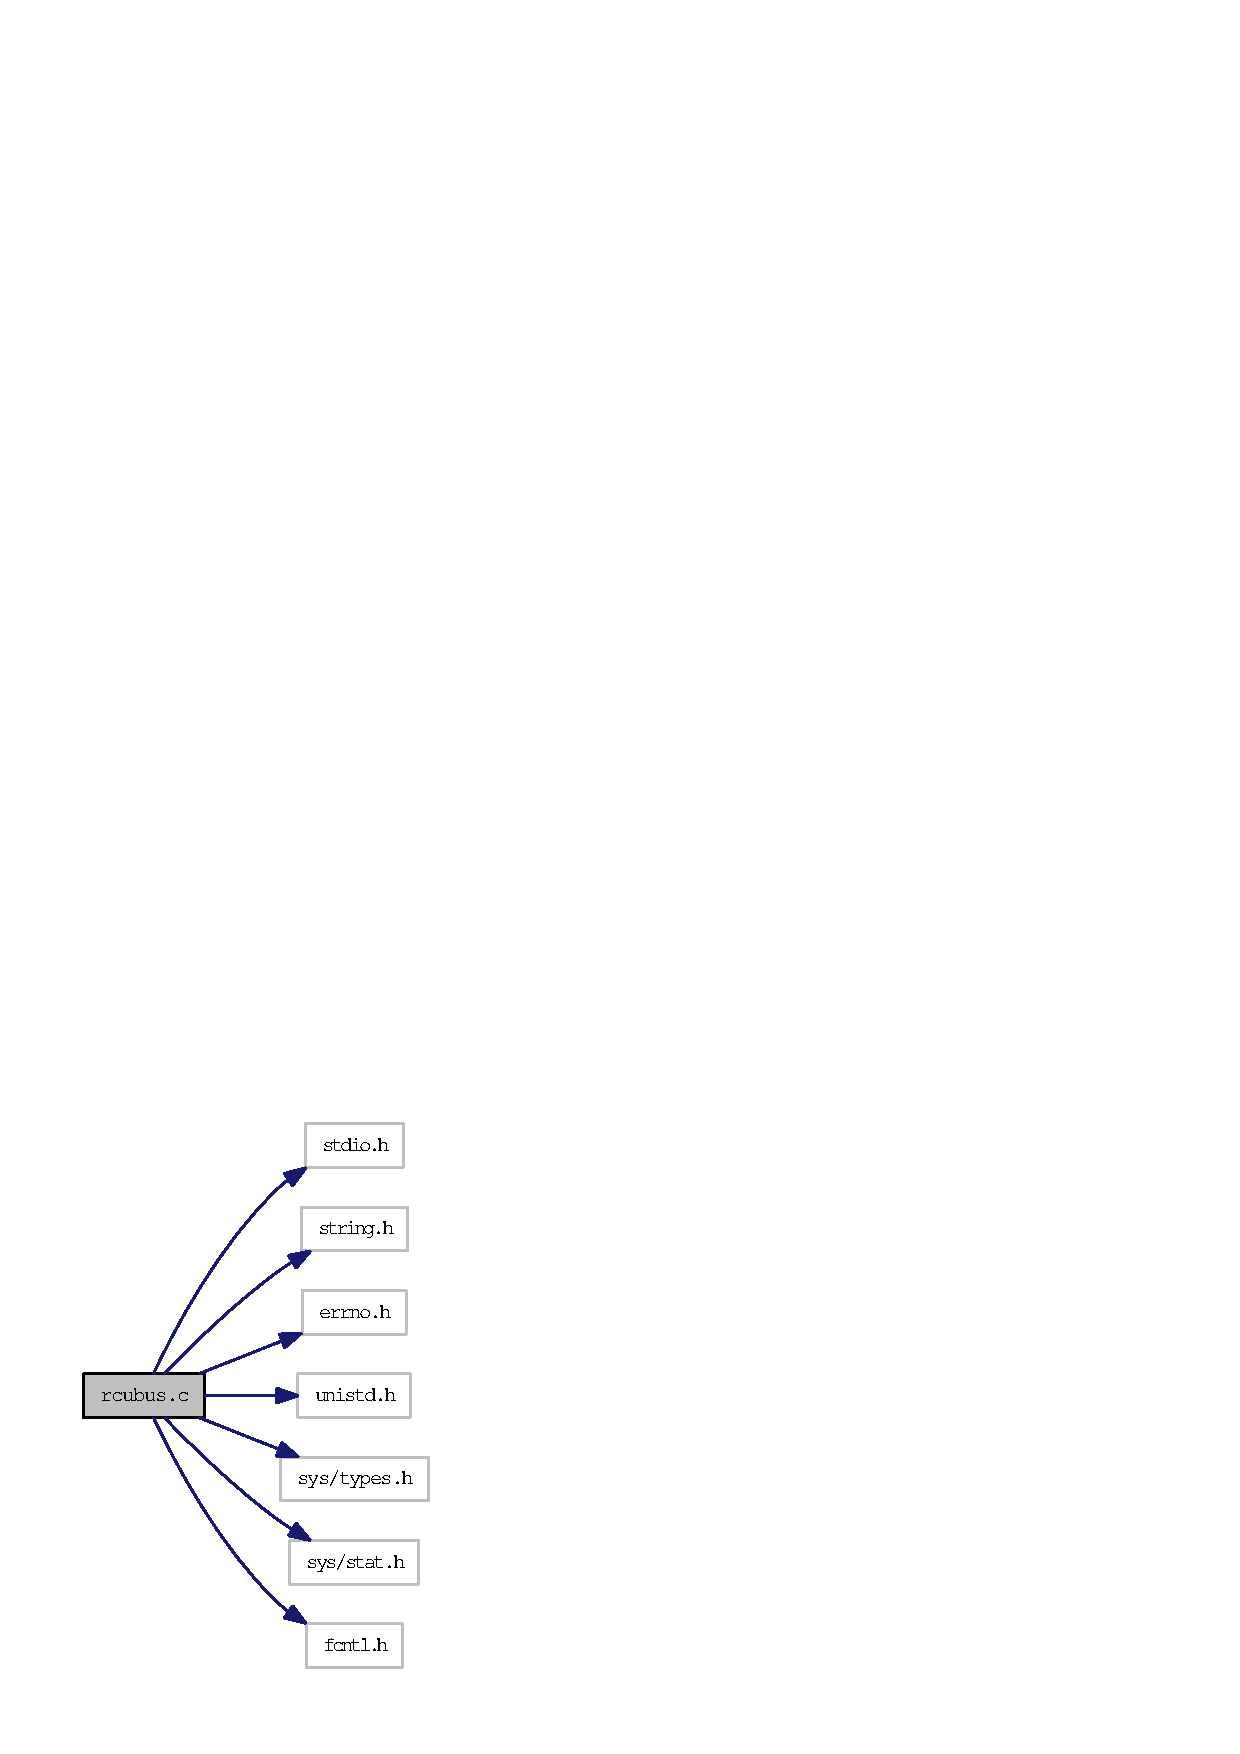
\includegraphics[width=105pt]{rcubus_8c__incl}
\end{center}
\end{figure}
\subsection*{Functions}
\begin{CompactItemize}
\item 
int \hyperlink{rcubus_8c_3c04138a5bfe5d72780bb7e82a18e627}{main} (int argc, char $\ast$$\ast$argv)
\end{CompactItemize}


\subsection{Function Documentation}
\hypertarget{rcubus_8c_3c04138a5bfe5d72780bb7e82a18e627}{
\index{rcubus.c@{rcubus.c}!main@{main}}
\index{main@{main}!rcubus.c@{rcubus.c}}
\subsubsection[main]{\setlength{\rightskip}{0pt plus 5cm}int main (int {\em argc}, char $\ast$$\ast$ {\em argv})}}
\label{rcubus_8c_3c04138a5bfe5d72780bb7e82a18e627}




Definition at line 13 of file rcubus.c.